\chapter{相關文獻討論}
\label{c:2}

%==========================================================================================
\section{第一階層子標題}

各階層子標題均應置於左側,並於其下方不空行。


引用文獻  ~\cite{Parker:2013}。引用文獻 \cite{Hsiao:2018}。


%==========================================================================================
\subsection{第二階層子標題}

第二階層子標題之內文。

%==========================================================================================
\subsubsection{第三階層子標題}

第三階層子標題之內文。


%==========================================================================================


\begin{table}[h!]
  \centering
  \caption{表格的說明!!!}
  \label{tbl:myLboro}
  \begin{tabular}{ | m{4.5cm} | m{4.5cm} | m{5.5cm} | }
    \hline
    研究團隊 & \centering 代表圖示  & 文獻探討 \\
    %------------------------------------------------------
    \hline
    %------------------------------------------------------
    \begin{minipage}{.25\textwidth}
      ~ \\ 加州大學 柏克萊分校 BAIR 實驗室 \\ 
      
\includegraphics[width=1.9cm]{fig/Isola2017/Isola.jpg} 
      
\includegraphics[width=1.9cm]{fig/Isola2017/Zhu.jpg}
      
\includegraphics[width=1.9cm]{fig/Isola2017/Zhou.png} 
      
\includegraphics[width=1.9cm]{fig/Isola2017/Efros.jpg}
      Isola 助理教授, MIT \\
      Zhu 助理教授, 卡內基美隆 \\      
      Zhou 博士生, Berkeley \\
      Efros 教授, Berkeley
    \end{minipage}
    &
    %\begin{minipage}[t]{5cm}
      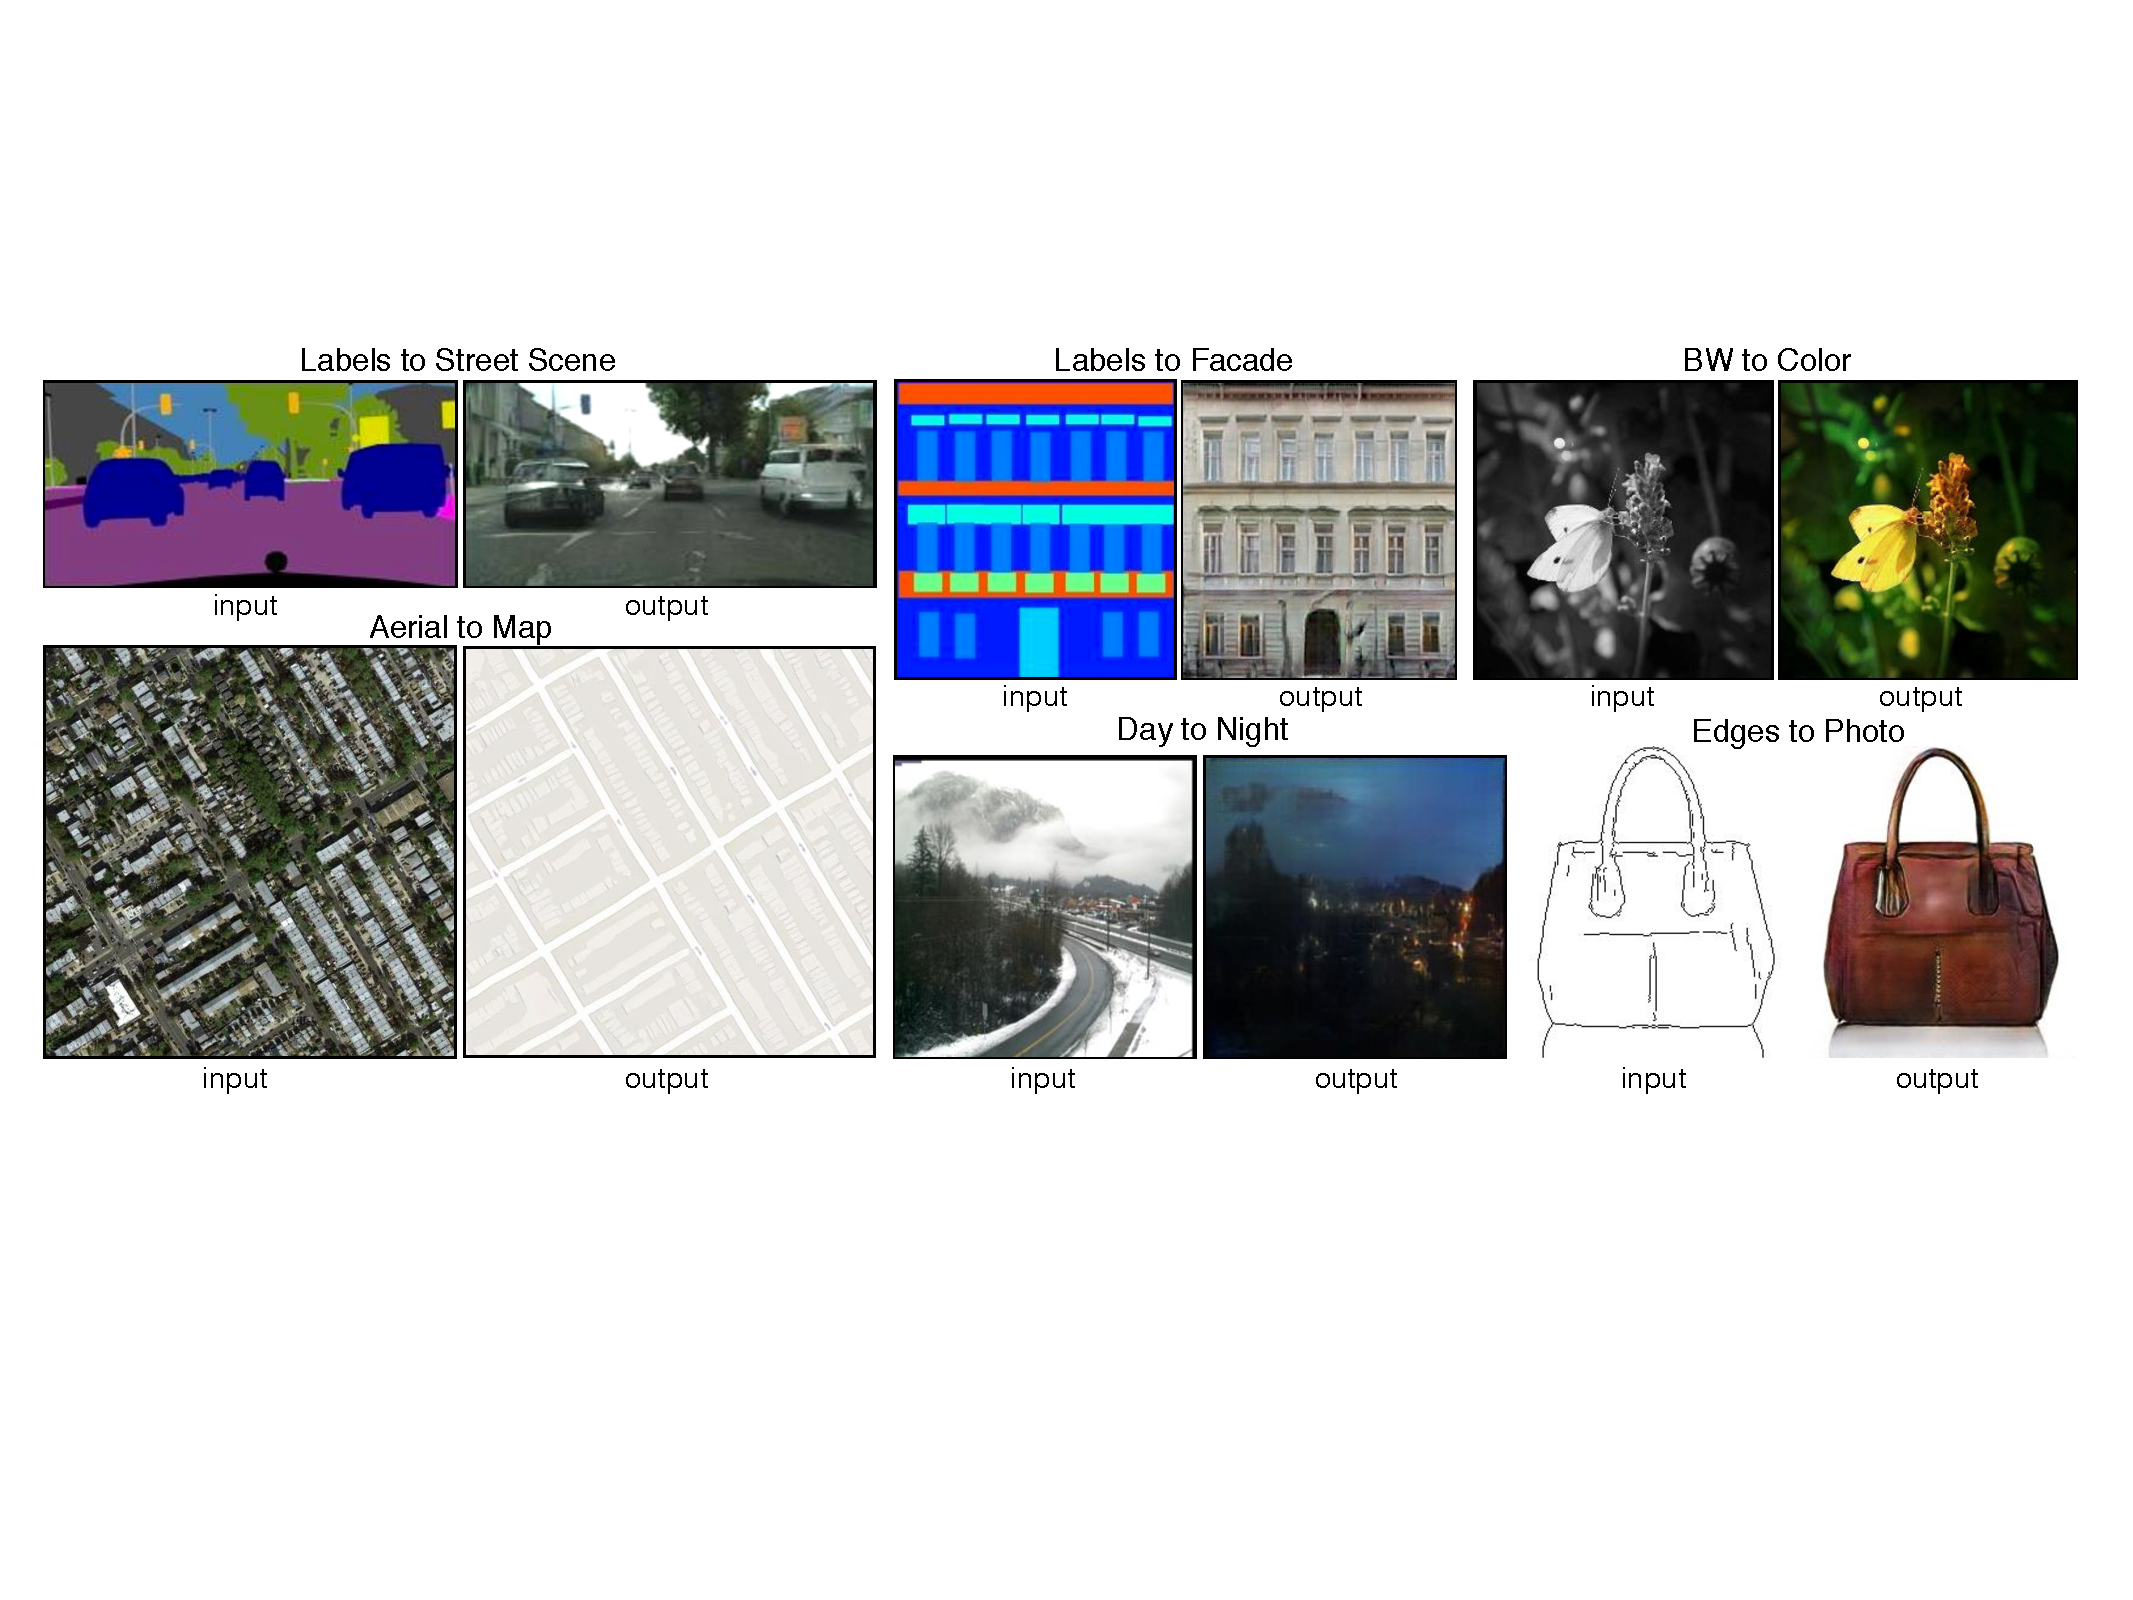
\includegraphics[width=4.3cm]{fig/Isola2017/teaser_v3.pdf}
      (圖片來源:~\cite{Isola2017})
    %\end{minipage}
    & 
    %\begin{minipage}{5cm}
      參考文獻 \cite{Isola2017} 
      該論文...
    %\end{minipage}
    %------------------------------------------------------ 
    \\ \hline
    %------------------------------------------------------
    ~ & ~ & ~
    %------------------------------------------------------ 
    \\ \hline
    %------------------------------------------------------
    ~ & ~ & ~
    %------------------------------------------------------ 
    \\ \hline
    %------------------------------------------------------
    ~ & ~ & ~
    %------------------------------------------------------ 
    \\ \hline
    %------------------------------------------------------
  \end{tabular}
\end{table}